% Generated by pysimcount.pffig13ext -- do not edit; regenerate instead.
% figure: fig13ext-rz -- Childs et al. 2018 Fig. 13 right, extended to every formula; diamonds before, circles after optimisation
% metric=rz gatebase=cz unmerged; r_method=measured-fit: r = ceil(a n^b) fitted to measured r, mean over seeds [1, 2, 3, 4, 5, 6, 7, 8, 9, 10], n = [5, 6, 7, 8, 9, 10, 11]; every point extrapolated
% optimised = Light reconstruction r x marginal + edge; verified n <= 16
% figure made at git_commit=3f419fd078cbd27a6e57919468bd4e5f1b96c08b git_dirty=False
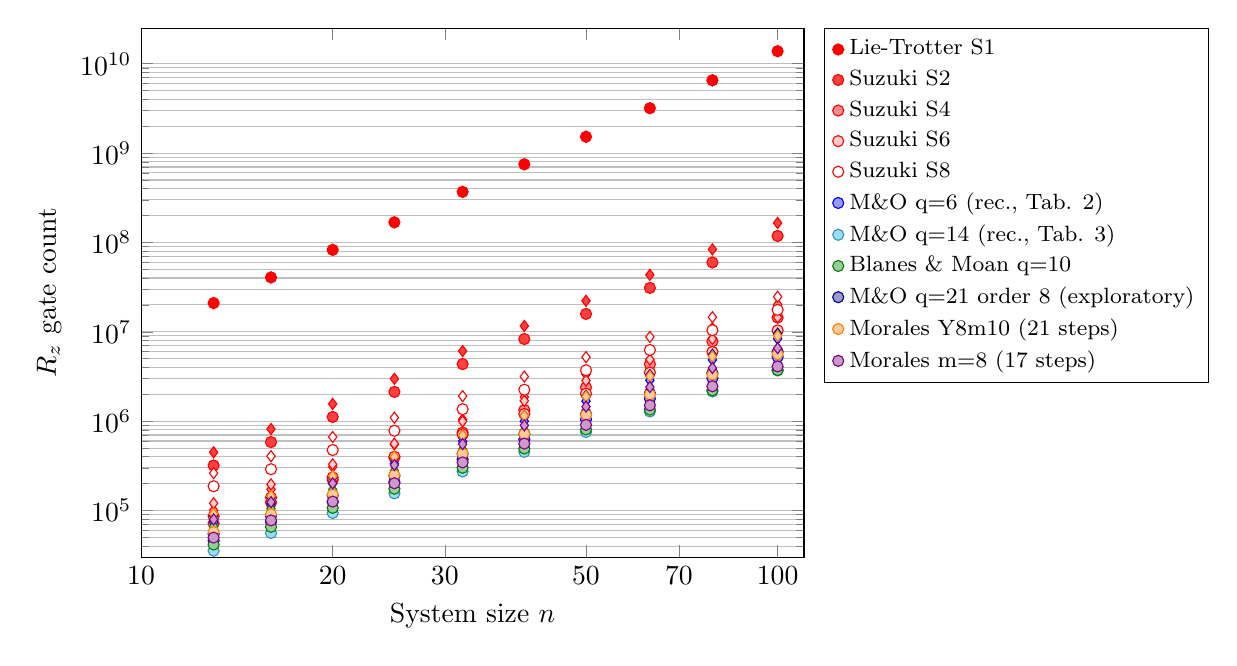
\begin{tikzpicture}
  \begin{loglogaxis}[
    width=10cm, height=8.3cm,
    xlabel={System size $n$}, ylabel={$R_z$ gate count},
    xmin=10, xmax=110,
    ymin=30000, ymax=2.5e+10,
    xtick={10,20,30,50,70,100}, xticklabels={10,20,30,50,70,100},
    ymajorgrids=true, yminorgrids=true,
    legend pos=outer north east, legend cell align=left,
    legend style={font=\footnotesize},
  ]
    \addplot[only marks, mark=*, mark size=2pt, draw=red, fill=red] coordinates {
      (13,20983456)
      (16,40624512)
      (20,82627040)
      (25,168057000)
      (32,368605440)
      (40,749714880)
      (50,1524861600)
      (63,3181082688)
      (79,6535652304)
      (100,13835801600)
    };
    \addlegendentry{Lie-Trotter S1}
    \addplot[only marks, mark=diamond*, mark size=2pt, draw=red, fill=red, forget plot] coordinates {
      (13,20983456)
      (16,40624512)
      (20,82627040)
      (25,168057000)
      (32,368605440)
      (40,749714880)
      (50,1524861600)
      (63,3181082688)
      (79,6535652304)
      (100,13835801600)
    };
    \addplot[only marks, mark=*, mark size=2pt, draw=red, fill=red!75] coordinates {
      (13,319683)
      (16,583616)
      (20,1114320)
      (25,2127650)
      (32,4351552)
      (40,8309040)
      (50,15865800)
      (63,31002363)
      (79,59743434)
      (100,118312600)
    };
    \addlegendentry{Suzuki S2}
    \addplot[only marks, mark=diamond*, mark size=2pt, draw=red, fill=red!75, forget plot] coordinates {
      (13,447538)
      (16,817040)
      (20,1560020)
      (25,2978675)
      (32,6092128)
      (40,11632600)
      (50,22212050)
      (63,43403220)
      (79,83640697)
      (100,165637500)
    };
    \addplot[only marks, mark=*, mark size=2pt, draw=red, fill=red!45] coordinates {
      (13,71838)
      (16,123216)
      (20,220020)
      (25,393150)
      (32,746432)
      (40,1333040)
      (50,2381300)
      (63,4342338)
      (79,7819104)
      (100,14427600)
    };
    \addlegendentry{Suzuki S4}
    \addplot[only marks, mark=diamond*, mark size=2pt, draw=red, fill=red!45, forget plot] coordinates {
      (13,100555)
      (16,172480)
      (20,308000)
      (25,550375)
      (32,1044960)
      (40,1866200)
      (50,3333750)
      (63,6079185)
      (79,10946635)
      (100,20198500)
    };
    \addplot[only marks, mark=*, mark size=2pt, draw=red, fill=red!20] coordinates {
      (13,86138)
      (16,140016)
      (20,235020)
      (25,400025)
      (32,712032)
      (40,1205040)
      (50,2031300)
      (63,3496563)
      (79,5954704)
      (100,10375100)
    };
    \addlegendentry{Suzuki S6}
    \addplot[only marks, mark=diamond*, mark size=2pt, draw=red, fill=red!20, forget plot] coordinates {
      (13,120575)
      (16,196000)
      (20,329000)
      (25,560000)
      (32,996800)
      (40,1687000)
      (50,2843750)
      (63,4895100)
      (79,8336475)
      (100,14525000)
    };
    \addplot[only marks, mark=*, mark size=2pt, draw=red, fill=white] coordinates {
      (13,186888)
      (16,290016)
      (20,475020)
      (25,781275)
      (32,1360032)
      (40,2250040)
      (50,3718800)
      (63,6260688)
      (79,10418204)
      (100,17625100)
    };
    \addlegendentry{Suzuki S8}
    \addplot[only marks, mark=diamond*, mark size=2pt, draw=red, fill=white, forget plot] coordinates {
      (13,261625)
      (16,406000)
      (20,665000)
      (25,1093750)
      (32,1904000)
      (40,3150000)
      (50,5206250)
      (63,8764875)
      (79,14585375)
      (100,24675000)
    };
    \addplot[only marks, mark=*, mark size=2pt, draw=blue, fill=blue!40] coordinates {
      (13,46033)
      (16,74416)
      (20,124820)
      (25,209275)
      (32,371552)
      (40,624040)
      (50,1047050)
      (63,1791783)
      (79,3031309)
      (100,5241100)
    };
    \addlegendentry{M\&O q=6 (rec., Tab. 2)}
    \addplot[only marks, mark=diamond*, mark size=2pt, draw=blue, fill=blue!40, forget plot] coordinates {
      (13,73632)
      (16,119040)
      (20,199680)
      (25,334800)
      (32,594432)
      (40,998400)
      (50,1675200)
      (63,2866752)
      (79,4849968)
      (100,8385600)
    };
    \addplot[only marks, mark=*, mark size=2pt, draw=cyan!70!black, fill=cyan!40] coordinates {
      (13,35503)
      (16,56016)
      (20,93820)
      (25,155775)
      (32,273312)
      (40,453640)
      (50,756050)
      (63,1283373)
      (79,2151249)
      (100,3689100)
    };
    \addlegendentry{M\&O q=14 (rec., Tab. 3)}
    \addplot[only marks, mark=diamond*, mark size=2pt, draw=cyan!70!black, fill=cyan!40, forget plot] coordinates {
      (13,56784)
      (16,89600)
      (20,150080)
      (25,249200)
      (32,437248)
      (40,725760)
      (50,1209600)
      (63,2053296)
      (79,3441872)
      (100,5902400)
    };
    \addplot[only marks, mark=*, mark size=2pt, draw=green!50!black, fill=green!50!black!40] coordinates {
      (13,41613)
      (16,65616)
      (20,107020)
      (25,175025)
      (32,300832)
      (40,494040)
      (50,807550)
      (63,1345113)
      (79,2216029)
      (100,3735100)
    };
    \addlegendentry{Blanes \& Moan q=10}
    \addplot[only marks, mark=diamond*, mark size=2pt, draw=green!50!black, fill=green!50!black!40, forget plot] coordinates {
      (13,66560)
      (16,104960)
      (20,171200)
      (25,280000)
      (32,481280)
      (40,790400)
      (50,1292000)
      (63,2152080)
      (79,3545520)
      (100,5976000)
    };
    \addplot[only marks, mark=*, mark size=2pt, draw=blue!50!black, fill=blue!50!black!40] coordinates {
      (13,54613)
      (16,87376)
      (20,147020)
      (25,244150)
      (32,430112)
      (40,718240)
      (50,1202300)
      (63,2050713)
      (79,3459094)
      (100,5953600)
    };
    \addlegendentry{M\&O q=21 order 8 (exploratory)}
    \addplot[only marks, mark=diamond*, mark size=2pt, draw=blue!50!black, fill=blue!50!black!40, forget plot] coordinates {
      (13,87360)
      (16,139776)
      (20,235200)
      (25,390600)
      (32,688128)
      (40,1149120)
      (50,1923600)
      (63,3281040)
      (79,5534424)
      (100,9525600)
    };
    \addplot[only marks, mark=*, mark size=2pt, draw=orange, fill=orange!40] coordinates {
      (13,57343)
      (16,90736)
      (20,151220)
      (25,249400)
      (32,433472)
      (40,718240)
      (50,1181300)
      (63,1991178)
      (79,3318079)
      (100,5638600)
    };
    \addlegendentry{Morales Y8m10 (21 steps)}
    \addplot[only marks, mark=diamond*, mark size=2pt, draw=orange, fill=orange!40, forget plot] coordinates {
      (13,91728)
      (16,145152)
      (20,241920)
      (25,399000)
      (32,693504)
      (40,1149120)
      (50,1890000)
      (63,3185784)
      (79,5308800)
      (100,9021600)
    };
    \addplot[only marks, mark=*, mark size=2pt, draw=violet, fill=violet!40] coordinates {
      (13,49738)
      (16,77536)
      (20,125820)
      (25,201900)
      (32,345472)
      (40,561040)
      (50,909550)
      (63,1504818)
      (79,2457769)
      (100,4097100)
    };
    \addlegendentry{Morales m=8 (17 steps)}
    \addplot[only marks, mark=diamond*, mark size=2pt, draw=violet, fill=violet!40, forget plot] coordinates {
      (13,79560)
      (16,124032)
      (20,201280)
      (25,323000)
      (32,552704)
      (40,897600)
      (50,1455200)
      (63,2407608)
      (79,3932304)
      (100,6555200)
    };
  \end{loglogaxis}
\end{tikzpicture}
